\documentclass{article}
\usepackage{amsmath}
\usepackage{graphicx}
\author{Kevin Lu, Travis You}
\title{Simulation and Inference for the Generalized Toilet Paper Problem}
\begin{document}
\maketitle
\section{Introduction}
In 1984, Knuth formulated a theoretical consideration for a ``toilet paper problem" \cite{Knuth1984}, which is a generalized matchbox problem from \cite{Feller}. 

Consider two types of people using a 2-roll toilet paper set: big-choosers and little-choosers. Big-choosers only uses toilet paper on the roll with more toilet paper and little-choosers only use toilet paper on the roll with less toilet paper. If both rolls have exactly the same amount of toilet paper, both types of people will randomly select a roll to use. Assume that all persons take 1 unit of toilet paper each time they use the restroom and that both rolls initially have $n$ units of toilet paper. If the amount of paper on the other roll when one roll is emptied is large, then the janitor would have plenty of time for replacement, but if that is not the case, people may run into problems.

Assume people enter the toilet independently at random, with proportion $p$ being big-choosers and proportion $q=1-p$ being little-choosers. Let $X$ be the random variable recording the number of paper left on one roll when the other roll first empties, Knuth showed that the expected value $E(X)$, denoted as $M_n(p)$, follows
\begin{equation}
    M_n(p) = n-\sum_{k=1}^{n-1} (n-k)c_k p^k q^{k-1}, 
\end{equation}
where $c_n = \binom{2n-2}{n-1}\frac{1}{n}$ is the catalan number. He has also given approximation of $M_n(p)$ for large $n$ as 
\begin{equation}
    M_n(p)=
    \begin{cases}
        \frac{q-p}{q}n+\frac{p}{q-p}+O(r^n) & \text{if }  p<1/2 \\
        \frac{p}{p-q} + O(r^n) & \text{if } p>1/2
    \end{cases}
    ,
    \label{limiting Mnp}
\end{equation}
where $r$ is any value greater than $4pq,$ which is smaller than $1$ for any $p \neq \frac{1}{2}$. The approximation in Eq.\eqref{limiting Mnp} works well when $|p-\frac{1}{2}|$ is at least of order $1/\sqrt{n}$. In that case, as $n$ is big, $O(r^n)$ is essentially 0. 

When $p$ is sufficiently close to $\frac{1}{2}$, the approximation in Eq.\eqref{limiting Mnp} does not work and $M_n(p)$ is better approximated by 
\begin{equation}
    M_n(p)=
    2\sqrt{\frac{n}{\pi}} - \frac{1}{4} \sqrt{\frac{1}{\pi n}} + O(n^{-3/2})
    \label{limiting Mnp equal}
\end{equation}

Therefore, when little-choosers predominate, $M_n(p)$ is of order $n$; when big-choosers predominate, $M_n(p)$ is of order $1$; when little-choosers and large-choosers are of similar number, $M_n(p)$ is of order $\sqrt{n}$. Moreover, there is a significant drop near $p=\frac{1}{2}$ for large $n$. 

In this paper, we're going to investigate further about the distribution of leftover amount $X$. Moreover, we're going to generalize the problem into a problem involving 3 and more rolls of toilet paper to test the claim that ``to solve the shortage of toilet paper when all other rolls empties, we just need to pile more rolls of toilet papers in the restroom.''
\section{2-Roll Problem}
Random-walk simulation is made to study the distribution of leftover toilet paper X, as described in the following. Two integers $i$ and $k$ are initialized to the same value $n$, representing the initial size of toilet paper in each roll. A number is randomly generated from a uniform distribution of [0,1). If the number is less than $p$, then the larger number between $i$ and $k$ is subtracted by 1. If not, then the smaller number between $i$ and $k$ is subtracted by 1. If $i$ and $k$ are equal, then either of the two is randomly chosen to be subtracted by 1. This process of choosing a number and subtracting 1 is continued, each time with a new random number from [0,1), until one of $i$ and $k$ becomes 0. The value of the nonzero number is recorded as X, giving a 1-time random-walk simulation (code implementation in Appendix A). 

To study the distribution of $X$, histogram of leftover paper size is drawn using 4000 simulations with $n=100$ at three different $p$, as shown in Fig.\ref{2roll-Histogram}.
\begin{figure}[ht]
    \centering
    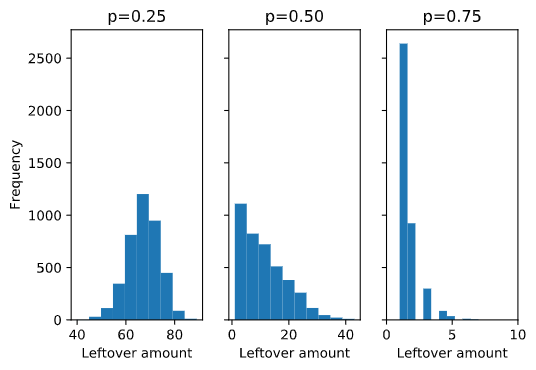
\includegraphics[width=10cm]{hist-2roll.png}
    \caption{Histogram of leftover paper size X with size 4000 at $p=0.25$ (left), $p=0.50$ (middle), and $p=0.75$ (right).}
    \label{2roll-Histogram}
\end{figure}
The shape of the distribution of leftover toilet paper size are different at different $p$, although all are unimodal. For $p<0.50$ (not too close to $0.50$), the distribution are approximately normal; for other cases, the distribution are skewed to the right and the right-skewness increases as $p$ increases. Center and variability will be discussed later using Fig.\ref{2roll-Mnp}.

In \cite{Knuth1984}, Knuth mainly discussed the expected value of leftover toilet paper size $M_n(p)$ and its approximate value when $n$ is large using Eq.\eqref{limiting Mnp} and Eq.\eqref{limiting Mnp equal}. As shown in Fig.\ref{2roll-approximation}, except for the horizontal line in the middle whose distance decreases as $n$ increases, the red and blue line are indistinguishable from each other. Therefore, the approximation in Eq.\eqref{limiting Mnp} and Eq.\eqref{limiting Mnp equal} work quite well at least for $n \geq 10$ for $p$ that deviates from $1/2$ with distance of order greater than $1/\sqrt{n}$. For $p$ that is sufficiently close to $1/2$, Eq.\eqref{limiting Mnp equal} provides a good estimation for the average value of $M_n(p)$ over this interval.
\begin{figure}[ht]
    \centering
    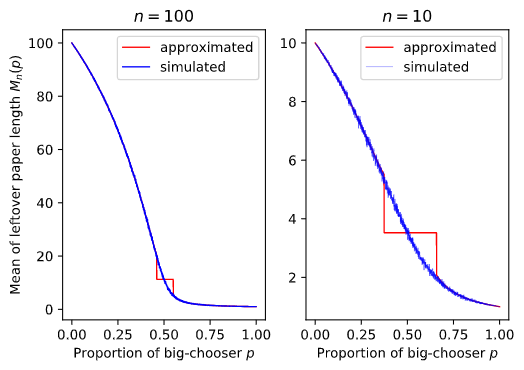
\includegraphics[width=10cm]{approxim-2roll.png}
    \caption{Comparison between approximated value in \cite{Knuth1984} and simulation result for computing expected value of leftover toilet paper size $M_n(p)$ at $n=100$ and $n=10$.}
    \label{2roll-approximation}
\end{figure} 

To further investigate center and variability of distribution for leftover toilet paper size, error band of $\bar{x} \pm 2s_x$ is drawn for three different initial toilet paper size $n$, where $\bar{x}$ is sample mean of $X$ and $s_x$ is sample standard deviation of $X$, as shown in Fig.\ref{2roll-Mnp}. The center of distribution (indicated by mean) initially starts form $O(n)$ and decreases gradually, then it decreases rapidly in the neighborhood of $p=0.5$ and quickly drops down to $O(1)$ after $p=0.6$. The variability, indicated by width of the error band, started small but grows quickly. After $p=0.6$, as in the case of center, the standard deviation drops down quickly $O(1)$. It should be noted that although skewness of distribution, as shown in Fig.\ref{2roll-Histogram}, makes mean a less accurate measure of center, the difference between curve showing mean of $X$ and median of $X$ at different $p$ is not significant. This is most likely because the skewness does not appear until $p \geq 1/2$, where the center has quickly descended to $O(1)$, making the difference less significant. In this paper, sample mean is preferred over median as a measure of center because accurate mathematical expression for $M_n(p)$ and its accurate approximation Eq.\eqref{limiting Mnp} and Eq.\eqref{limiting Mnp equal} are handy. Moreover, it is easier to carry out inference using sample mean instead of median.
\begin{figure}[ht]
    \centering
    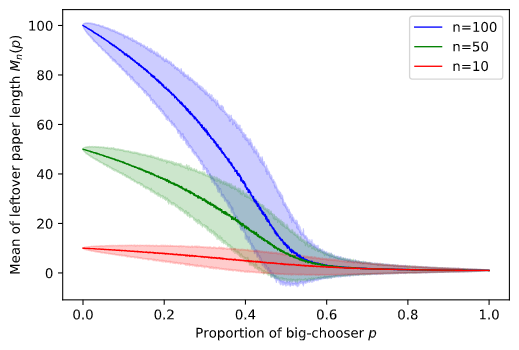
\includegraphics[width=10cm]{Mnp-2roll.png}
    \caption{Expected value of leftover toilet paper size $M_n(p)$ verses big-chooser proportion $p$ with error band of width 2 sample standard deviation at $n=10$, $n=50$, and $n=100$.}
    \label{2roll-Mnp}    
\end{figure}
\bibliographystyle{unsrt}
\bibliography{MyCollection.bib}
\end{document}